\documentclass{article}


\usepackage[english]{babel}
\usepackage[utf8]{inputenc}

\usepackage{kotex}

\usepackage[top=2cm,bottom=2cm,left=3cm,right=3cm,marginparwidth=1.8cm]{geometry}



\usepackage{tikz}
\usepackage{stanli}
\usepackage{commath,amsmath}
\usepackage{xcolor}
\usepackage{subcaption}
\usepackage{graphicx}
\usepackage{tikz}
\usepackage{tikzpagenodes}

\usetikzlibrary{calc,patterns,through,angles,quotes}


\makeatletter
\newcommand*\bigcdot{\mathpalette\bigcdot@{.5}}
\newcommand*\bigcdot@[2]{\mathbin{\vcenter{\hbox{\scalebox{#2}{$\m@th#1\bullet$}}}}}
\makeatother

\begin{document}
\title{Four bar(4절 링크)}
\author{B817145 최원준}
\maketitle

\section{분석 및 예상 결과}


\begin{figure}[h]
\begin{subfigure}[h]{.5\linewidth}
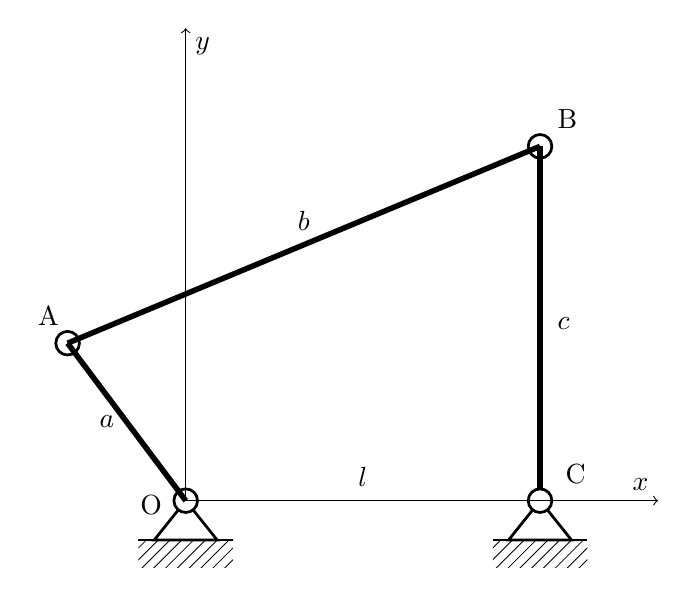
\begin{tikzpicture}[scale=1, transform shape]

\point{o}{0}{0};
\point{first}{-0.7}{-0.3};
\notation{1}{first}{O};
\support{1}{o};
\hinge{1}{o};

\point{a}{-1.5}{2};
\point{first}{-2}{2.1};
\notation{1}{first}{A};
\hinge{1}{a};
\beam{4}{a}{o};

\point{b}{4.5}{4.5};
\point{first}{4.6}{4.6};
\notation{1}{first}{B};
\hinge{1}{b};
\beam{4}{a}{b};

\point{c}{4.5}{0};
\point{first}{4.7}{0.1};
\notation{1}{first}{C};
\support{1}{c};
\beam{4}{c}{b};
\hinge{1}{c};

\draw [->] (0,0) -- (6,0) node [above left]  {$x$};
\draw [->] (0,0) -- (0,6) node [below right] {$y$};
\node at (-1,1) {$a$};
\node at (1.5,3.55) {$b$};
\node at (4.8,2.25) {$c$};
\node at (2.25,0.3) {$l$};

\end{tikzpicture}
\subcaption{초기 상태(t=0)} \label{fig:M1}
\end{subfigure}
\begin{subfigure}[h]{.7\linewidth}
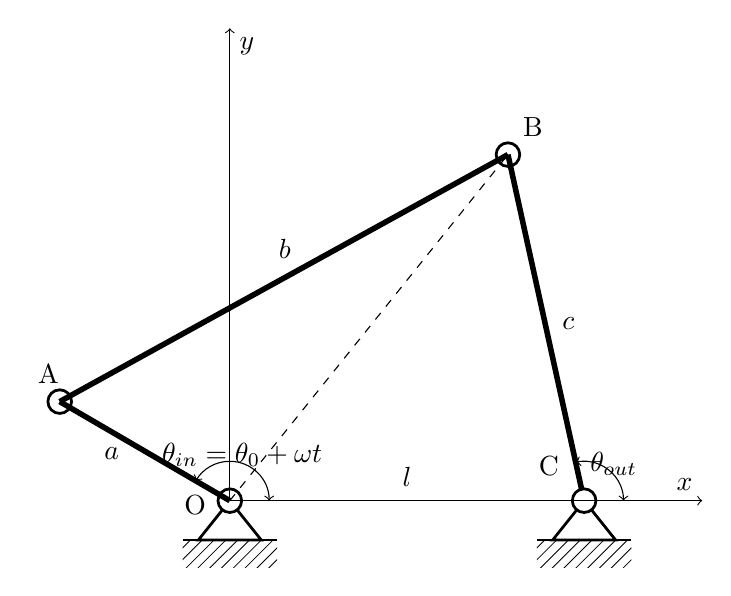
\begin{tikzpicture}[scale=1, transform shape]

\point{o}{0}{0};
\point{first}{-0.7}{-0.3};
\notation{1}{first}{O};
\support{1}{o};
\hinge{1}{o};

\point{a}{-2.16}{1.258};
\point{first}{-2.56}{1.358};
\notation{1}{first}{A};
\hinge{1}{a};
\beam{4}{a}{o};

\point{b}{3.5325}{4.3948};
\point{first}{3.6}{4.5};
\notation{1}{first}{B};
\hinge{1}{b};
\beam{4}{a}{b};

\point{c}{4.5}{0};
\point{first}{3.8}{0.2};
\notation{1}{first}{C};
\beam{4}{c}{b};
\support{1}{c};
\hinge{1}{c};

\draw [->] (0,0) -- (6,0) node [above left]  {$x$};
\draw [->] (0,0) -- (0,6) node [below right] {$y$};


\node at (-1.5,0.6) {$a$};
\node at (0.7,3.2) {$b$};
\node at (4.3,2.25) {$c$};
\node at (2.25,0.3) {$l$};

\coordinate (O) at (0,0);
\coordinate (A) at (-2.16, 1.258);
\coordinate (B) at (3.5325, 4.3948);
\coordinate (C) at (4.5, 0);
\coordinate (cprime) at (1, 0);
\coordinate (X) at (5.6, 0);

\draw [dashed] (o) -- (b);

\pic["$\theta_{in}=\theta_0+\omega t$",draw=black,<->,angle eccentricity=1.2,angle radius=0.5cm] {angle=cprime--O--A};
\pic["$\theta_{out}$",draw=black,<->,angle eccentricity=1.2,angle radius=0.5cm] {angle=X--C--B};

\end{tikzpicture}
\subcaption{시간 t가 지난 후의 모습} \label{fig:M1}
\end{subfigure}
\end{figure}


\subsection{자유도 해석}
$\theta_{in}$이 결정되면, $\overline{OB}$가 정해지고 $\triangle OBC$ 가 유일한
삼각형으로 결정된다. 따라서 $\theta_{in}$이 결정되는 순간 4절 링크 $OABC$는 구속된다. 그러므로 자유도는 0이다.



\subsection{관계식 유도}
\noindent시간 t에서 4절 링크의 운동에 대해 분석해보자.\\

\noindent(i) 주어진 점 $B$의 속도에 대한 식을 유도한다. (단, $\theta_{in}=\theta_0+\omega t$ ,   $\frac{d\theta_{out}}{dt}=\omega_{CB}=\omega_{out}$ 이다.)
\begin{align*} 
A : r_A &= < a\cos\theta_{in} ,\,a\sin\theta_{in}> \\
B : r_B &= < l + c \cos \theta_{out},\,c\sin\theta_{out}> \\
 v_B &= v_C + \omega_{out} \times r_{B/C} = \omega_{out} \times r_{B/C}\\
 &= v_A + \omega_{AB} \times r_{B/A}\\
 &= < -a\sin\theta_{in} ,\,a\cos\theta_{in}>\bigcdot\,\omega + \omega_{AB} \times < l + c \cos \theta_{out} -a\sin\theta_{in},\,c\sin\theta_{out} -a\cos\theta_{in}> \\
 &= < -\omega\, a\sin\theta_{in} -\omega_{out}\, c\sin\theta_{out} +\omega_{out}\, a\cos\theta_{in},\, \omega\, a\cos\theta_{in} + \omega_{AB}\, l + \omega_{AB} \,c \cos\theta_{out} -\omega_{AB}\, a\sin\theta_{in}>\\
 &= \frac{dr_B}{dt} = < -c\sin\theta_{out} , \,c\cos \theta_{out} >\bigcdot\,\omega_{out}\\ 
\end{align*}

\par위의 식을 통해 다음과 같은 연립방정식을 얻을 수 있다.\\
\begin{equation}
\begin{cases}
\omega_{out} \,c\sin\theta_{out} = \omega\bigcdot\, a\sin\theta_{in} + \omega_{AB}\bigcdot\,(c\sin\theta_{out}-a\sin\theta_{in})\\
\omega_{out} \,c\cos\theta_{out} = \omega\bigcdot\, a\cos\theta_{in} + \omega_{AB}\bigcdot\,(l + c\cos\theta_{out}-a\cos\theta_{in})
\end{cases}
\end{equation}
\\ \\*




(ii) $\theta_{in}$와 $\theta_{out}$의 관계\\

\begin{figure}[h]\centering
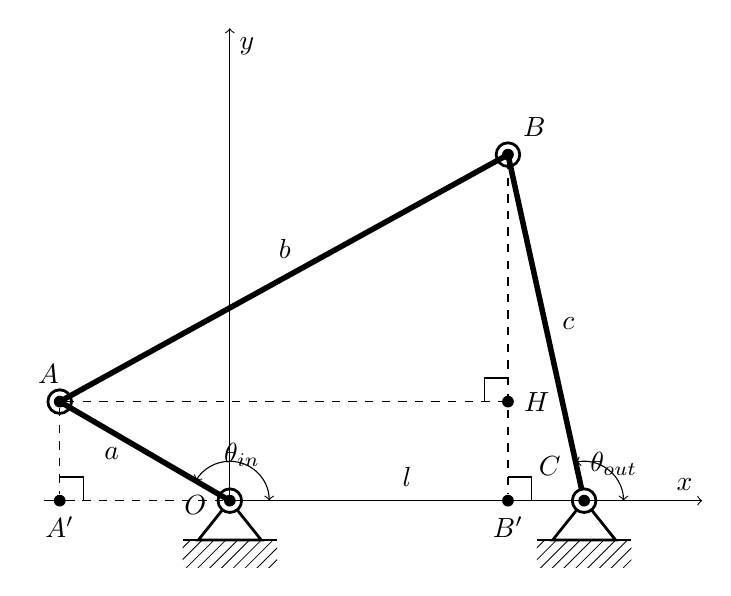
\begin{tikzpicture}[ dot/.style={circle,fill,inner sep=1.5pt}][scale=1, transform shape]
\point{o}{0}{0};
\point{first}{-0.7}{-0.3};
\notation{1}{first}{$O$};
\support{1}{o};
\hinge{1}{o};

\point{a}{-2.16}{1.258};
\point{first}{-2.56}{1.358};
\notation{1}{first}{$A$};
\hinge{1}{a};
\beam{4}{a}{o};

\point{b}{3.5325}{4.3948};
\point{first}{3.6}{4.5};
\notation{1}{first}{$B$};
\hinge{1}{b};
\beam{4}{a}{b};

\point{c}{4.5}{0};
\point{first}{3.8}{0.2};
\notation{1}{first}{$C$};
\beam{4}{c}{b};
\support{1}{c};
\hinge{1}{c};

\draw [->] (0,0) -- (6,0) node [above left]  {$x$};
\draw [->] (0,0) -- (0,6) node [below right] {$y$};


\node at (-1.5,0.6) {$a$};
\node at (0.7,3.2) {$b$};
\node at (4.3,2.25) {$c$};
\node at (2.25,0.3) {$l$};

\coordinate (O) at (0,0);
\coordinate (A) at (-2.16, 1.258);
\coordinate (B) at (3.5325, 4.3948);
\coordinate (C) at (4.5, 0);
\coordinate (cprime) at (1, 0);
\coordinate (X) at (5.6, 0);

\pic["$\theta_{in}$",draw=black,<->,angle eccentricity=1.2,angle radius=0.5cm] {angle=cprime--O--A};
\pic["$\theta_{out}$",draw=black,<->,angle eccentricity=1.2,angle radius=0.5cm] {angle=X--C--B};
\draw  (-2.36,0) -- (-1.96,0);


\coordinate (aprime) at (-2.16,0);
\draw(aprime) coordinate[dot,label=below:$A^\prime$] (aprime);
\coordinate (bprime) at (3.5325,0);
\draw(bprime) coordinate[dot,label=below:$B^\prime$] (bprime);
\coordinate (h) at (3.5325, 1.258);
\draw(h) coordinate[dot,label=right:$H$] (h);

\draw(o) coordinate[dot] (o);
\draw(a) coordinate[dot] (a);
\draw(b) coordinate[dot] (b);
\draw(c) coordinate[dot] (c);

\draw [dashed] (o) -- (aprime);
\draw [dashed] (a) -- (aprime);
\draw [dashed] (b) -- (bprime);
\draw [dashed] (a) -- (h);

\pic [draw,angle radius=0.3cm] {right angle = o--aprime--a};
\pic [draw,angle radius=0.3cm] {right angle = a--h--b};
\pic [draw,angle radius=0.3cm] {right angle = b--bprime--c};


\end{tikzpicture}
\end{figure}

\begin{quote}
    $A$에서 $x$축에 내린 수선의 발을 $A`$, $B$에서 $x$축에 내린 수선의 발을 $B`$라 하자.\\
    또한, $A$에서 $\overline{BB`}$에 내린 수선의 발을 $H$라 하면 다음과 같이 쓸 수 있다.\\*
    \begin{align*}
        \overline{AA^\prime} &= a\sin\theta_{in}\\
        \overline{BB^\prime} &= c\sin\theta_{out}\\
        \overline{BH} &= \overline{BB^\prime} - \overline{AA^\prime} = c\sin\theta_{out} - a\sin\theta_{in}\\
        \overline{AH}^2 \!\!&= \overline{AB}^2 - \overline{BH}^2 \;\;\;\;\;\;\; \overline{AH}=\sqrt{b^2 -(c\sin\theta_{out}-a\sin\theta_{in})^2}\\
        \overline{OC}&=\overline{AH}-\overline{OA^\prime}+\overline{B^\prime C}\\
    \end{align*}
    따라서 다음과 같은 관계를 얻는다.\\\\*
    \begin{equation}
    l=\sqrt{b^2 -(c\sin\theta_{out}-a\sin\theta_{in})^2}+a\cos\theta_{in}-c\cos\theta_{out}
    \end{equation}
 \\*
\end{quote}


(iii)
\begin{quote}
    (ii)의 식(2)에 의해 특정 시간 $t$에서 $\theta_{in}$가 결정되면, $\theta_{out}$를 구할 수 있다. 따라서 (i)의 식(1)은 2-변수 연립방정식이 되어 $\omega_{out}$와 $\omega_{AB}$를 구하기에 충분하다.
\end{quote}
    
\pagebreak
    
\section{결과값 비교}
\noindent직접 계산한 값과 \verb+adams+ 프로그램으로 구한 물리량을 비교하자.\\\\*
\indent1의 $l, a, b, c$, $\omega_{in}$, $t$, $\theta_0$를 다음과 같이 설정하자\\*
\begin{align*}
	l&=180 & \omega_{in}&=1\,(rad/s)\\
	a&=100 & \theta_0&=2.214\,(rad)\\
	b&=260 & t&=0.4\,(s)\\
	c&=180 \,(cm \;\;unit)
\end{align*}\\

\subsection{직접 계산}
\indent section 1.2의 식(2)와 (1)에 대입하면 다음과 같다.\\
\begin{align*}
    \theta_{in}&=2.214+1\bigcdot\,0.4=2.614\,(rad)\\
    180&=\sqrt{260^2 -(180\sin\theta_{out}-100\sin(2.614))^2}+100\cos(2.614)-180\cos\theta_{out}
\end{align*}\\
\indent다음을 얻는다.\\
\begin{equation*}
    \theta_{out}=1.7878\,(rad)\;\;\;(\frac{\pi}{2}<\theta_{out}<\pi)
\end{equation*}\\

\indent 또한 식(1)에서
\begin{equation*}
\begin{cases}
\omega_{out}\bigcdot\,180\,\sin(1.7878) = 100\,\sin(2.614) + \omega_{AB}\bigcdot\,(180\,\sin(1.7878)-100\,\sin(2.614))\\
\omega_{out}\bigcdot\,180\,\cos(1.7878) = 100\,\cos(2.614) + \omega_{AB}\bigcdot\,(180+180\,\cos(1.7878)-100\,\cos(2.614))\\
\end{cases}
\end{equation*}\\

\indent따라서 $\omega_{out}$, $\omega_{AB}$는 다음과 같다.
\begin{align*}
    \omega_{out}&=0.497\,(rad/s)\\
    \omega_{AB}&=0.295\,(rad/s)
\end{align*}
\pagebreak
\subsection{adams로 구한 값}

주어진 4절 링크를 다음과 같이 구현.\\
\begin{figure}[h]
\begin{subfigure}{\textwidth}
  \centering
  % include first image
  \includegraphics[width=.9\linewidth]{fourbar.PNG}  
  \caption{adams로 구현한 4절 링크}
  \label{fig:sub-first}
 \end{subfigure}\\
 \begin{subfigure}{\textwidth}
  \centering
  % include first image
  \includegraphics[width=.9\linewidth]{graph.PNG}  
  \caption{물리량 해석 graph}
  \label{fig:sub-first}
 \end{subfigure}\\*
\begin{subfigure}{.5\textwidth}
  \centering
  % include first image
  \includegraphics[width=.8\linewidth]{result2.PNG}  
  \subcaption{$Y\,:\,\omega_{out}$}
  \label{fig:sub-first}
 \end{subfigure}
 \begin{subfigure}{.5\textwidth}
  \centering
  % include first image
  \includegraphics[width=.8\linewidth]{result1.PNG}  
  \subcaption{$Y\,:\,\omega_{AB}$}
  \label{fig:sub-first}
 \end{subfigure}
\end{figure}\\
\indent직접 계산한 값과 거의 유사한 값을 얻었다.
\pagebreak

\section{손해석 및 손계산 첨부}
\begin{figure}[h]
 \begin{subfigure}{\textwidth}
  \centering
  % include first image
  \includegraphics[width=\linewidth]{hand1.jpg}  
  \caption{손 해석}
  \label{fig:sub-first}
 \end{subfigure}
 \begin{subfigure}{\textwidth}
  \centering
  % include first image
  \includegraphics[width=\linewidth]{hand2.jpg}  
  \caption{손 계산}
  \label{fig:sub-first}
 \end{subfigure}
 \end{figure}
 \footnote{\LaTeX{}\LaTeX{}\LaTeX{}\LaTeX{}\LaTeX{}\LaTeX{}\LaTeX{}\LaTeX{}\LaTeX{}\LaTeX{}\LaTeX{}\LaTeX{}\LaTeX{}\LaTeX{}\LaTeX{}\LaTeX{}\LaTeX{}\LaTeX{}\LaTeX{}\LaTeX{}\LaTeX{}}

\end{document}
